\section{Background}\label{s:background}

\subsection{Student Rocketry}
High-powered Rocketry (HPR) involves the design, construction, and launching of rockets that operate with thrust levels higher than those of model rocketry. University student teams have adopted HPR as a platform for practical aerospace engineering education, competing in events such as the Spaceport America Cup and the European Rocketry Challenge (EuRoC), where rockets target altitudes of up to 9\,km while carrying scientific payloads \cite{rocketpy-ref}.

A typical HPR flight consists of three phases. The first is powered flight, in which the motor burns and the rocket accelerates upward. Once the propellant is exhausted, the rocket enters a coasting phase, continuing to ascend until it reaches its maximum altitude, known as the apogee. Finally, a parachute system is deployed to slow the rocket for safe recovery \cite{rocketpy-ref}. 

Before launch, teams typically rely on trajectory simulation tools to verify rocket designs and predict performance. OpenRocket~\cite{niskanen2013openrocket} is commonly used for initial rocket design, while higher fidelity tools such as Ironbark \cite{galletly2026ironbark} and RocketPy~\cite{rocketpy-ref} are used where a more accurate prediction of the trajectory and apogee is required.

\subsection{Flight Software}

Flight software is central to HPR operations. It is responsible for acquiring sensor data, detecting flight phases and executing all critical events throughout a rocket's trajectory~\cite{clary2024georgia-tech-avionics}. At minimum, the recovery system consists of a drogue parachute deployed first at apogee to stabilise the descent, followed by a larger main parachute deployed at a predetermined altitude~\cite{Jasztal-drogue-main-parachute}. More advanced flight computers also implement active control systems. One such system is drag-based apogee control via air-brake mechanisms. This involves controlling motor-driven flaps during the coasting phase to increase aerodynamic drag, reducing the rocket's velocity, and allowing the flight computer to precisely target a desired apogee altitude~\cite{sophie-evaluation-various-airbrake}.



\subsection{F Prime Framework}
Traditionally, flight software has been tightly coupled with mission-specific hardware, making code reuse between projects difficult. F Prime is an open-source flight software framework developed at NASA's Jet Propulsion Laboratory (JPL) that addresses this problem by prioritising modularity and portability across hardware architectures~\cite{canham2022fprime-mars-helicopter, bocchino2018fprime, bocchino2022fpp}. It targets small-scale embedded systems such as CubeSats and SmallSats, and has been flight-proven across several missions at NASA, including the ASTERIA CubeSat and, most notably, the Ingenuity Mars Helicopter, which completed a series of successful autonomous flights on Mars in 2021~\cite{canham2022fprime-mars-helicopter}. 

\subsubsection{Components}
Every F Prime project is composed of components that behave similarly to classes in object-oriented languages in that they encapsulate state and behaviour. However, unlike classes, they have no symbolic dependencies and do not interact with each other; all communication is driven through typed interfaces called ports. Components can be of three distinct types. Passive components have no thread or message queue and are driven entirely by the thread of the calling component. Queued components add a message queue, allowing invocations to be carried over for processing on another thread. Active components extend this further with their own dedicated thread, independently dequeuing and processing messages~\cite{canham2022fprime-mars-helicopter, bocchino2018fprime, bocchino2022fpp}.


\subsubsection{Topologies}
A topology in F Prime defines the wiring of the system, specifically the port connections between component instances, which are resolved at deployment time~\cite{canham2022fprime-mars-helicopter, bocchino2018fprime, bocchino2022fpp}. Since topologies are defined separately from the components themselves, different topologies can be defined from the same set of components for different deployment targets. In the context of this study, this enables the flight topology and the simulation topology to share flight software components while replacing hardware drivers with simulated counterparts.


\subsection{RocketPy Simulator}\label{background-rocketpy}
RocketPy is an open-source Python library first introduced by Ceotto et al. \cite{rocketpy-ref} in 2021. It implements a 6-degree-of-freedom simulator that tracks translational and rotational motion across three axes, accounting for variable mass effects as propellant is consumed during the burn phase and descent under parachutes. The library is structured into four main classes: Environment, Motor, Rocket and Flight. Each class exposes various configurable options, allowing the end user to fully customise the simulation by adjusting the rocket's geometry, mass, aerodynamic coefficients, thrust curve and the environmental conditions at the launch site. RocketPy has been formally adopted as a competition requirement by the European Rocketry Challenge (EuRoC), which requires teams to submit a RocketPy simulation file as part of their application. % cite euroc rules

Numerical integration works by advancing the simulation in small discrete time steps, approximating the state of the rocket at $X_{t+1}$ based on the forces and moments acting on it in the current state $X_t$ \cite{gautschi2011numerical}. By default, RocketPy uses the LSODA solver, which automatically switches between two internal integration methods based on the behaviour of the equations of motion. This is especially useful in rocket trajectory simulations, as some phases of flight evolve smoothly, while others involve rapidly changing dynamics that require smaller integration steps to sustain accuracy.

RocketPy provides limited support for integrating user-defined flight software into the simulation loop. It exposes a controller interface where a single callback function can be registered per controlled component, such as air brakes or parachutes \cite{soares2022rocketpy}. These functions are invoked at a configurable sampling rate, receiving the current simulation state and returning a control output that influences the rocket's behaviour. By default, RocketPy enables \texttt{time\_overshoot}, a configurable parameter that allows the integrator to use optimised step sizes and step past scheduled time nodes. Disabling this parameter forces the integrator to stop at every controller time node, making controller execution strictly discrete. Separately from the controller's sampling rate, the Flight class also exposes the solver's step sizes via the \texttt{max\_time\_step} and \texttt{min\_time\_step} parameters~\cite{soares2022rocketpy, rocketpy-docs-airbrakes}. Both the callback sampling rate and these solver step parameters are treated as independent variables later in this study in Section \ref{variable-selection}.


RocketPy also provides built-in sensor models for accelerometers, gyroscopes and barometers. These models simulate the physical characteristics of each sensor, converting simulation state variables into sensor readings that can be consumed by flight software as if they were received by hardware. In this study, these models were used to enable the F Prime flight software to operate on realistic sensor-derived estimates rather than simulation state variables.


\subsection{Simulation-Based Flight Software Verification}
Simulation-based verification applies a closed feedback loop between the flight software and a mathematical model of the physical system, known as the plant, as illustrated in Figure~\ref{fig:simulation-diagram}. The flight software receives sensor readings and computes outputs that feed back to the plant model, thus advancing the simulation state and driving the evolution of the modelled system~\cite{ulbig2019flightsimulatorbasedverification}.
RocketPy serves as the plant model in this setup, while F Prime acts as the Flight Software.

\begin{figure}[h]
    \centering
    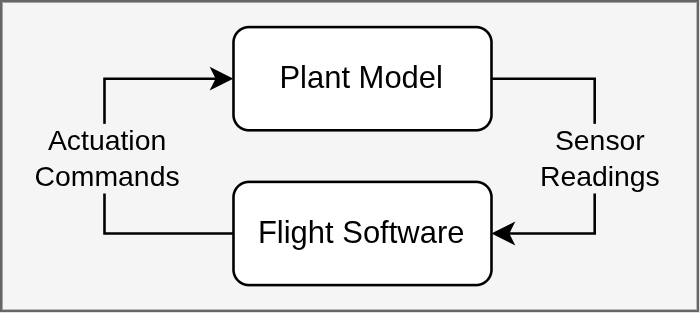
\includegraphics[width=0.5\textwidth]{figures/simulation verification.drawio.png}
    \caption{Closed-loop simulation-based verification, showing the data exchange between the plant model and flight software.}
    \label{fig:simulation-diagram}
\end{figure}


The fidelity of this approach depends on how closely the plant model captures the real vehicle's dynamics and on whether the software executes on a host machine or the actual flight hardware \cite{ulbig2019flightsimulatorbasedverification, kiesbye2019-moveII-cubsat}. Two methodologies reflect this tradeoff: Software-in-the-Loop (SIL) and Hardware-in-the-Loop (HIL).

In SIL testing, the system under test and the plant model are executing on the same host under common time \cite{ulbig2019flightsimulatorbasedverification}. This makes SIL fast to set up and well-suited to early development, where the goal is to validate software logic before committing to hardware. In HIL testing, the flight software is deployed and executed on the actual target hardware, while the plant model continues to run on a separate host machine~\cite{kiesbye2019-moveII-cubsat, santos-hil-uav-autopilot}. Sensor data is transmitted to the hardware, and control outputs are returned over a physical interface, introducing real-time behaviour, latency and hardware-specific execution constraints that SIL cannot capture. This makes HIL a higher-fidelity verification step, confirming that the software behaves correctly not just in logic but under the timing and resource constraints of the real flight hardware.



\subsection{Co-Simulation}
Co-Simulation encompasses the theory and techniques for coupling independent simulators, each advancing its own internal state, to achieve a global simulation \cite{gomes2017cosimulation}. Each simulator acts as a black box, interacting only through exchanges of inputs and outputs at synchronisation points separated by a communication step size $H$ \cite{gomes2017cosimulation}.

Simulators in Co-Simulation theory may be continuous-time, integrating a set of differential equations internally between communication steps, or discrete, advancing only when triggered by an external event \cite{gomes2017cosimulation}.  This distinction is central to the coupling problem addressed in this thesis. RocketPy is a continuous-time simulator, while F Prime flight software executes as a discrete, event-driven process. The way the two are coupled at their synchronisation boundary is described in Section~\ref{closed-loop-sim-env}.


